\documentclass[a4paper]{article}

%\usepackage[margin=2cm]{geometry}
%\usepackage{qtree}
%\usepackage{color}
%\usepackage{forest}
\usepackage{listings}
\usepackage{tikz}	%for the graphics
\usepackage{cite} 	%for bibtex
\usepackage{url}	%for the url's in bibtex



\begin{document}
\begin{titlepage}
	\begin{center}
		\begin{figure}[t]
			\centering
			
\includegraphics[width=350px]{logo.PNG}
		\end{figure}
		
		\begin{center}
			\textsc{\Huge Programming Languages}
		\end{center}
		\begin{center}
			\textsc{\Huge COS 333}
		\end{center}
		\begin{center}		
			\textsc{\LARGE Practical Lab Experience 1:}		
		\end{center}
		\begin{center}		
			\textsc{\LARGE Research Assignment}		
		\end{center}
		
		\begin{flushright} \large
			Juan Jaques du Preez \newline \emph{u15189016} \newline
		\end{flushright}
\par\vspace{\fill}
{\large Date:}
\\
{\large \today}

	\end{center}
\end{titlepage}

\tableofcontents
\newpage

\section{Question 1: Esolang}
According to esolangs.org \cite{esolang}, an esoteric programming language, or esolang, is a computer programming language that is designed to experiment with peculiar ideas and to be a joke, rather than for practical use. The word \textit{esoteric} means "likely to be understood by only a small number of people\cite{wikipedia}." This implies that such a language would only be understood and used by a smaller population, as it was created to be vastly different from normal programming languages. 
\section{Question 2: Views on Esoteric languages}
	\subsection{Argument against}
	Although esoteric languages have been considered as no more than jokes, they do seem to carry some potential. This potential may not be to write practical programs, or even to be used in the real world, but there are other possibilities to consider when thinking about these languages. First of all, it stimulates creative and lateral thinking. Wikipedia\cite{wikipedia2} explains that \textit{lateral thinking} means "an indirect method of thinking which is not immediately obvious and involves ideas which may not be obtainable by using the traditional step-by-step method of thinking." This "out of the box" means of thought introduces brand new ideas to solving problems, which may turn out useful in computer science research. These problem solving methods could be a big aid to test the boundaries and limits of our current knowledge of computer science, as well as information science.
	
	Also, these esolangs can be thought of as an expression of creativity; it can be seen as form of art\cite{esolangArt}. Some of these languages are no more useful than a painting hanging in a gallary. The general premise is that the creators made such a difficult language simply because they can. This happens in the same way a water-colour painting is a representation of the artist's abilities and talents. The programming language of Piet is a good example of this, as it transforms each program into a literal work of modern art. (see figure 1)
	
	\subsection{Argument for}	
	However, it must be said that some esoteric languages are specifically just for fun. For example, the language LOLCODE is based on the LOLCats phenomenon\cite{esolangArt}. It uses silly words and phrases that would commonly be used by LOLCats to write programs. A lot of this could be seen as a waste of time. These programmers could have spent their time doing formal research into some computer science prinicples instead of playing around with silly features. One could have seen a better furthering of research if their time spent were more focused. 
	
			\begin{figure}[h]
			\centering
			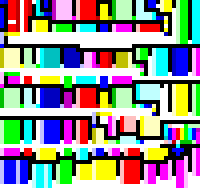
\includegraphics[width=200px]{helloworld-piet.png}
			\caption{Piet Hello World Program}
		\end{figure}
\section{Question 3: Practical Examples}
	\subsection{Esolang one: Ook!}	
	Ook! is an esoteric language based on another esoteric language called BrainF***. It was created by a man called David Morgan-Mar even before the year 2008. Both of these languages are Turing-complete\cite{ook2}. How the program achieves this is by the means of moving a pointer around in an array, and changing the values in the array at the pointer address. There are only three distinct syntax elements in Ook!:
	\begin{itemize}
	\item Ook.
	\item Ook?
	\item Ook!
	\end{itemize}
	These three elements are combined to form the eight commands of its BrainF***counterpart. These eight commands have the following properties: \cite{ook}
\begin{itemize}

    \item Ook. Ook?\\
    Move the Memory Pointer to the next array cell.
    \item Ook? Ook.\\
    Move the Memory Pointer to the previous array cell.
    \item Ook. Ook.\\
    Increment the array cell pointed at by the Memory Pointer.
    \item Ook! Ook!\\
    Decrement the array cell pointed at by the Memory Pointer.
    \item Ook. Ook!\\
    Read a character from STDIN and put its ASCII value into the cell pointed at by the Memory Pointer.
    \item Ook! Ook.\\
    Print the character with ASCII value equal to the value in the cell pointed at by the Memory Pointer.
    \item Ook! Ook?\\
    Move to the command following the matching Ook? Ook! if the value in the cell pointed at by the Memory Pointer is zero. Note that Ook! Ook? and Ook? Ook! commands nest like pairs of parentheses, and matching pairs are defined in the same way as for parentheses.
    \item Ook? Ook!\\
    Move to the command following the matching Ook! Ook? if the value in the cell pointed at by the Memory Pointer is non-zero. 
\end{itemize}	
	The code lacks a lot in the readability and writability departments, as there are only three different possibilities of lexical tokens.
	\begin{lstlisting}
Ook. Ook? Ook. Ook. Ook. Ook. Ook. Ook. Ook. Ook. Ook. 
Ook. Ook. Ook. Ook. Ook. Ook. Ook. Ook. Ook. Ook! Ook?
Ook? Ook. Ook. Ook. Ook. Ook. Ook. Ook. Ook. Ook. Ook. 
Ook. Ook. Ook. Ook. Ook. Ook. Ook. Ook. Ook? Ook! Ook! 
Ook? Ook! Ook? Ook. Ook! Ook. Ook. Ook? Ook. Ook. Ook. 
Ook. Ook. Ook. Ook. Ook. Ook. Ook. Ook. Ook. Ook. Ook. 
Ook! Ook? Ook? Ook. Ook. Ook. Ook. Ook. Ook. Ook. Ook. 
Ook. Ook. Ook? Ook! Ook! Ook? Ook! Ook? Ook. Ook. Ook. 
Ook! Ook. Ook. Ook. Ook. Ook. Ook. Ook. Ook. Ook. Ook. 
Ook. Ook. Ook. Ook. Ook. Ook! Ook. Ook! Ook. Ook. Ook. 
Ook. Ook. Ook. Ook. Ook! Ook. Ook. Ook? Ook. Ook? Ook. 
Ook? Ook. Ook. Ook. Ook. Ook. Ook. Ook. Ook. Ook. Ook. 
Ook. Ook. Ook. Ook. Ook. Ook. Ook! Ook? Ook? Ook. Ook. 
Ook. Ook. Ook. Ook. Ook. Ook. Ook. Ook. Ook? Ook! Ook! 
Ook? Ook! Ook? Ook. Ook! Ook. Ook. Ook? Ook. Ook? Ook. 
Ook? Ook. Ook. Ook. Ook. Ook. Ook. Ook. Ook. Ook. Ook.
Ook. Ook. Ook. Ook. Ook. Ook. Ook. Ook. Ook. Ook. Ook! 
Ook? Ook? Ook. Ook. Ook. Ook. Ook. Ook. Ook. Ook. Ook. 
Ook. Ook. Ook. Ook. Ook. Ook. Ook. Ook. Ook. Ook. Ook. 
Ook? Ook! Ook! Ook? Ook! Ook? Ook. Ook! Ook! Ook! Ook! 
Ook! Ook! Ook! Ook. Ook? Ook. Ook? Ook. Ook? Ook. Ook? 
Ook. Ook! Ook. Ook. Ook. Ook. Ook. Ook. Ook. Ook! Ook. 
Ook! Ook! Ook! Ook! Ook! Ook! Ook! Ook! Ook! Ook! Ook! 
Ook! Ook! Ook. Ook! Ook! Ook! Ook! Ook! Ook! Ook! Ook! 
Ook! Ook! Ook! Ook! Ook! Ook! Ook! Ook! Ook! Ook. Ook. 
Ook? Ook. Ook? Ook. Ook. Ook! Ook. 
	\end{lstlisting}
	\subsection{Esolang two: Whenever}	
	Whenever is another interesting esoteric programming language created by David Morgan-Mar. The language is said to be turing complete. The idea behind Whenever is that the program does a list of tasks in whichever order it wants to. It definitely gets to each task, but does it whenever it feels like it. The syntax works as follows. A single item on the todo list is constructed by a line number followed by a statement. Statements can be forgotten, deferred, or done more than once. This is done with the keywords forget, defer, and again respectively. These keywords specify whether an item should be removed from the todo list, remain on the todo list after executing the line, or be done later.
	
	Here is an example of printing out the first 100 fibonacci numbers:
	\begin{lstlisting}
1 again (1) defer (3 || N(1)<=N(2) || N(7)>99) 2#N(1),3,7;
2 again (2) defer (3 || N(2)<=N(1) || N(7)>99) 1#N(2),3,7;
3 defer (5) print(N(1)+N(2));
4 defer (5) print("1");
5 4,-3,7;
6 defer (4) 3;
7 7;
8 defer (N(7)<100) -1#N(1),-2#N(2),-7#100,-3;
9 defer (3 || 6) 1,3; 
	\end{lstlisting}
\section{Question 4: Stack-based Programming Languages}
	A stack-based programming language is a language which makes use of an implicit stack or several stacks as a fundemental design for the language. It uses the pushing and popping qualities of the stack to pass parameters between operations and functions. 
	
	Take for example the programming language PostScript. As its name suggests, it uses post-fix notation to perform operations. To explain this, I will use the example of a function add(4,5). Infix notation portrays this mathematical operation as "4 + 5", but postfix notation shows it as "4 5 +." In a stack based programming language, the function would be "4 5 add." The programming language pushes 4 and 5 onto the stack. When "add" is read, the two numbers are popped off the stack, added together, and the result is pushed onto the stack again. So, the parameters, as well as the return values, for the "add" function are accessed from a single stack. These characteristics of the stack is used throughout the program, and among all the other functions.
\section{Question 5: Turing (the programming language)}
	From the special keywords and syntax, it is clear that Turing was designed to be very readable. The	use of words such as "begin," "end," "var," and "loop" suggest that it is imperative that the user understands what the program is doing at all times. It is expected that the programmer follows the programming logic when reading the code. It is good for teaching programming, because it portrays core programming principles in easy-to-understand pseudocode, which is designed to be close to natural language. Thus, the focus is on teaching the principles rather than the syntax of the language. A fully featured programming language like C++ or java has many syntax to remember, which ought not to be the focus when just starting with programming.
	
	However, as soon as one is familiar with the concepts of programming, one no longer has need for such an introductory language as Turing. It becomes redundant to write out "begin," "end," or "end if" every time when a single symbol would suffice. If you understand where a selection statement or loop begins and ends, and are used to the logic behind the syntax, then one might as well use the short-hand syntax.
	
	Also, in terms of the writability, the language is not so good. The language itself is not very powerful since it does not access memory directly or have my different libraries compared to more popular languages. Thus, one cannot always complete a certain task in Turing that one can complete using Java, for example, because there is simply no support for that kind of flexibility.
	
	
\section{Question 6: Design by Contract}
	According to \url{wiki.c2.com} \cite{c2}, Design by Contract (DbC) is "a software correctness methodology that uses preconditions and postconditions to document (or programmatically assert) the change in state caused by a piece of the program." In essence, formal interface specifications for software components are created in the form of "contracts," which contain these specifications of design. Quality control is a key element of Design by Contract. One achieves a certain quantifiable level of software quality by specifying obligations and expectations for the different components in the system.
	
	Eiffel (created in 1986) is one example of a porgramming language that conforms to the Design by Contract methodology. Eiffel was designed specifcally for the purpose of providing a reliable, formal language which can be used in industry, so the DbC methodology was perfect for this purpose. Software quality is essential to an Eiffel program. Another example that natively supports DbC is Cobra, which is used as a general pupose object-oriented programming language. 
	
\section{Question 7: AWK Programming Language}
	AWK is a programming language that is primarily used for text processing, data extraction, filtering, and writing reports. AWK works with streams of textual data and can perform operations on data as input from files or as part of a pipeline. These operations are concerned with pattern matching, formalising data, and providing a formatted report based on the resultant data.
	
	The general syntactic structure of AWK can be seen as a set of condition-action pairs which look like the following:
	\begin{lstlisting}
	condition { action }
	condition { action }
	\end{lstlisting}
	The conditions can be expressions, and are usually patterns. Patterns are formed with the use of regular expressions. Actions are commands or statements such as functions, calculations, or assignments. These actions are to be performed on the given data set.
	
	The use of regular expressions and patterns allow for textual data in the form of records and fields to be filtered, letting only the desired data remain. This is similar, in some regards, to an SQL statement that SELECTS only the fields and records that follow specific criteria. In the same way, this structure selects only particular data according to the patterns specified, and then performs certain operations on that data. This is perfect for the application because one uses only the particular subset of the data to perform operations and can easily save the results of the data processing into another file. Data selection is completely separate from the data processing, so one can have different functions working on the same set of data. On the other hand, one can have one function work on many different datasets.

\bibliography{mybib}{}
\bibliographystyle{plain}
	
\end{document}
